\documentclass[10pt]{sigplanconf}

\usepackage{amsmath}
\usepackage[T1]{fontenc}
\usepackage{url}
\usepackage{graphicx}


\begin{document}

\authorpermission
\conferenceinfo{OOPSLA'07,} {October 21--25, 2007, Montr{\'e}al, Qu{\'e}bec, Canada.} 
\CopyrightYear{2007} 
\copyrightdata{978-1-59593-786-5/07/0010}


\title{CUTE: C++ Unit Testing Easier}

\authorinfo{Peter Sommerlad\and Emanuel Graf}
           { IFS Institute for Software at HSR Rapperswil\\
Oberseestr. 10, CH-8640 Rapperswil, Switzerland}
           {\{peter.sommerlad,emanuel.graf\}@hsr.ch}

\maketitle

\begin{abstract}
This article describes the design and use of the CUTE C++ testing framework and its integration into the 
Eclipse C++ Development Tooling.

Unit testing supports code quality and is a corner stone of agile software development. CUTE and its 
Eclipse plug-in are an easy to use C++ testing framework.
\end{abstract}

\category{D}{2}{5}[Testing tools (e.g., data generators, coverage testing)]

\terms
Design, Languages, Verification

\keywords
Unit Testing, C++, Eclipse

\section{Introduction}
Automated unit testing supports high quality of program code, especially under inevitable change and 
refactoring. As a side effect, unit tested code often has a better structure. Java developers are 
used to unit testing because of JUnit and its tight integration into IDEs like Eclipse. C++ programmers 
lacked the tool support for easy-to-use unit testing, even though the language's complexity asks for it. 
Refactoring and simplifying C++ code without tests is very hard and error-prone.

\section{Problems with CPPUnit}
One disadvantage of the well-known CPPUnit is that you have to write a subclass to have your own test case.
Inheritance is a very strong coupling between classes. Requiring a test-case class to inherit from a 
CPPUnit-framework class couples both closely together. The CPPUnit tutorial \cite{CppUnitCookbook} lists 
at least six classes you have to deal with to get things up and running. You even have to decide if 
you want to inherit from TestCase or TestFixture for your simple test case you intend to write.

\section{Using CUTE}
Writing a unit test using CUTE is simple. A test is a simple parameterless void function, there is no 
need to inherit from a test class.
\begin{verbatim}
#include "cute.h"
int theAnswer = 42;

void mysimpletest(){
  ASSERT(theAnswer == 6*7);
}
\end{verbatim}
In addition each test has a name, which identifies it. That name is either given during 
construction using the CUTE() macro or derived from the function's typeid.

Running a single test is not very useful. But having a larger collection of test cases and 
running them  after every check-in on a build server, is what makes unit testing so powerful. So there is 
a need for running many tests at once.

CUTE doesn't use the Composite Design Pattern \cite{DesignPatterns} for implementing the container for 
these test cases. Instead test suites in CUTE are vectors containing a sequence of test cases. Thus we 
can avoid the strong coupling caused by inheritance and the lower cohesion in the container class, because 
the container doesn't need to support the composite interface. Test cases can be added to the suite using 
the \verb|push_back()| method inherited from vector or the overloaded \verb|+=| operator.

Since C++ lacks some of the reflection mechanisms available in Java, we have to write our own main 
function for testing. For simple cases we only instantiate a runner object and pass our test for 
execution.

Reporting the test results is so common that CUTE provides a means to configure the runner 
with a listener passed as template parameter.
\newpage
\begin{verbatim}
void runSuite(){
  cute::suite s;
  s.push_back(CUTE(mysimpletest));
  cute::ide_listener lis;
  cute::makeRunner(lis)(s, "The Suite");
}

int main(){
  runSuite();
}
\end{verbatim}

\section{Eclipse CDT Integration}
A good integration into a development environment simplifies the use of a testing framework. Additionally 
a good integration can improve the developers acceptance to write tests, so writing unit tests becomes 
a natural part of writing source code.

The CUTE Eclipse plug-in\footnote{Update Site: \url{http://ifs.hsr.ch/cute/updatesite/}} integrates the 
CUTE testing framework into the Eclipse C/C++ Development Tooling (CDT)
\footnote{\url{http://www.eclipse.org/cdt/}} similar to the JUnit integration for the Eclipse Java 
Development Tools\footnote{\url{http://www.eclipse.org/jdt/}}. The plug-in's project creation wizards 
support the developer by setting up a project including the necessary CUTE headers and the corresponding 
compiler and linker settings. A specialized wizard exists to create a test project for an already 
existing library project.

The plug-in uses the standard cute runner with a special output listener that writes the test results to 
\verb|std::cout| using a defined format. A model representing the test cases including there results is build
 by parsing the test output. The results of the tests are presented to the developer by the result view. Therefore the 
result view can be used with other test frameworks as long as they provide the same output as the 
\verb|cute::eclipse_listener|.

CUTE's result view provides all the important features Java developers know from the JUnit-plug-in:
\begin{itemize}
 \item Red / Green Bar
 \item test navigator
 \item diff-viewer for failing tests
\end{itemize}

\begin{figure}
 \begin{center}
 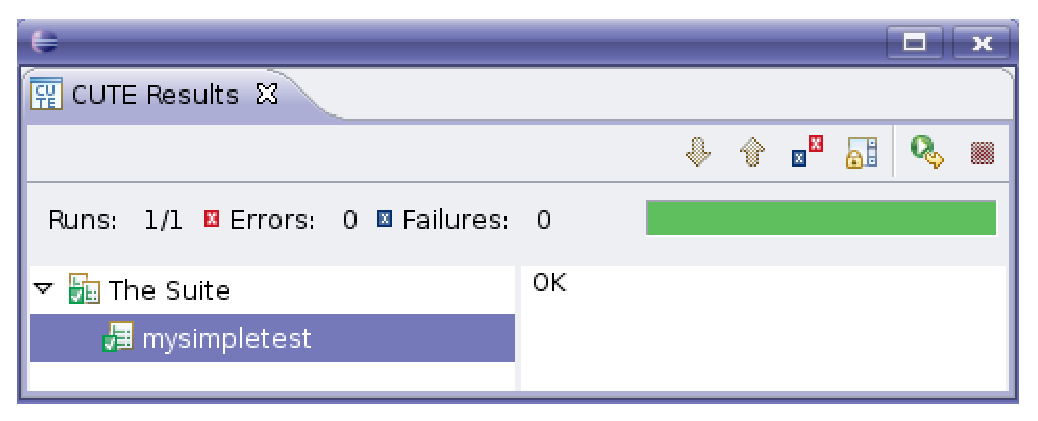
\includegraphics[width=0.45\textwidth]{results}
\end{center}
 \caption{CUTE Result View}
\label{result View}
\end{figure}

\section{Requirements and Outlook}
CUTE needs \verb|boost::bind| and \verb|boost::function| from the Boost\footnote{\url{http://www.boost.org/}} 
library that are part of the proposed C++ standard extension \verb|std::tr1|.

There are many ideas for extending CUTE to make it a more convenient environment to work with. 
For example, better integration into other IDEs like Visual Studio.

\begin{thebibliography}{}

\bibitem{CppUnitCookbook}
M.~Feathers and B.~Lepilleur.
\newblock Cppunit cookbook.
\newblock
  \url{http://cppunit.sourceforge.net/doc/lastest/cppunit_cookbook.html}.

\bibitem{DesignPatterns}
E.~Gamma, R.~Helm, R.~Johnson, and J.~Vlissides.
\newblock {\em Design Patterns}.
\newblock Addison-Wesley Professional, July 1997.

\end{thebibliography}

\end{document}
1-59593-090-6/05/0007